\documentclass[border=6pt]{standalone}
\usepackage{tikz}
\usepackage[edges]{forest}
\usetikzlibrary{arrows.meta,positioning,calc,decorations.pathreplacing,shapes.geometric}
\begin{document}
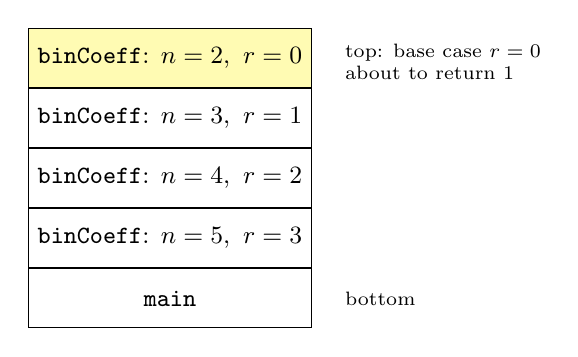
\begin{tikzpicture}[font=\small,rec/.style={draw,minimum width=3.6cm,minimum height=0.75cm,align=center}]
\node[rec] (m) at (0,0) {\texttt{main}};
\node[rec,above=0cm of m] (a) {\texttt{binCoeff}: $n=5,\ r=3$};
\node[rec,above=0cm of a] (b) {\texttt{binCoeff}: $n=4,\ r=2$};
\node[rec,above=0cm of b] (c) {\texttt{binCoeff}: $n=3,\ r=1$};
\node[rec,above=0cm of c,fill=yellow!30] (d) {\texttt{binCoeff}: $n=2,\ r=0$};
\node[font=\scriptsize,anchor=west] at (2.1,0) {bottom};
\node[font=\scriptsize,anchor=west,align=left] at (2.1,3.0) {top: base case $r=0$\\about to return 1};
\end{tikzpicture}
\end{document}
